
\chapter{Introduction}\paragraph{}Understanding the world around us is the goal of every scientist, from the chemist that experiments with the formation of atoms to the geologist exploring the process of rock formations. Nuclear physicists focus on studying the fundamental constituents of matter, the building blocks of nature. Physicist use scattering experiments at accelerator facilities, like CERN in Switzerland, DESY in Germany, BATES in Massachusetts, JLab in Virginia, and many others, to study the protons and neutrons that make up a nucleus and the constituents that form the internal structure of a nucleon. These experiments allow physicists to probe inside a nucleus to observe the internal structure and to investigate the interactions between the quarks and gluons. Many of the experiments are design to confirm an existing results while also expanding on unique ideas.
\paragraph{}In the last century, there have been numerous breakthroughs in the fields of nuclear and particle physics. Rutherford discovered the proton by bombarding light nuclei with alpha particles to produce the reaction,  
	\begin{equation}
	^{14}N + ^4He \rightarrow ^{17}O + p.
	\end{equation}
This reaction allowed Rutherford to conclude that the Hydrogen nucleus was a elementary constituent of atomic nuclei \cite{PnN}. In the late 1950s, experimental results published by W. McAllister and R. Hofstadter exposed some of the eternal structure of the proton \cite{Flay,Hof}. The European Muon Collaboration(EMC) produced results in the early 1980s showing a difference between the internal structure of the deuterium nucleus and Iron \cite{seeley,CC}. In the current era, scientific labs can produce beams of leptons, hadrons, and heavy ions. These beams can be produced with a large energy spread from "cold" neutrons of $10^{-2}eV$ to protons of $10^{12}eV$. The data received from scattering experiments using beams with a complex structure like alpha particles of heavy ions contain information about the target, the beam, and the interaction between the two. 
\paragraph{}This thesis will discuss using deep inelastic scattering to study the internal structure of two light nuclei and gain a better understanding of the effects of the slight difference between these two light nuclei as part of the E12-010-103 experiment. The discussion will include the motivations, approach, and the outcome from one analysis technique.

\section{Electron scattering}\label{sec:escat}
\paragraph{}Deciphering and analyzing data from scattering experiments that use complex beams can be convoluted because the scattering interaction contains information about the internal structure of the target and the beam along with the complex interactions and forces between the two \cite{PnN}.  In order to remove some of the complexity in scattering experiments, one may employ highly relativistic electrons. Electrons being point-like particles without any internal structure allow the elimination of some of the analysis difficulties due to the complex nature of the internal structure of more complex scattering tools. Electrons and the target either a nucleus, nucleon, or quark interact via the exchange of a virtual photon. Using quantum electrodynamics (QED), these interactions can accurately be described by the well known electromagnetic interaction.
\paragraph{}The electromagnetic interaction describes the coupling of fundamental particles via their electric charge. The interaction between two electrically charged particles begins when a virtual photon is emitted. The amplitude for the emission of photon is proportional to $\sqrt{\alpha}$. Where $\alpha$ is the fine structure constant. Higher order terms of this process contribute very little due to the coupling constant $\alpha \approx 1/137 $, being much smaller than one. 
\paragraph{} The Feynman diagram in figure \ref{feynman} represents an electron scattering from a proton. The incoming or incident electron's four-momentum is described as k = (E,$ \vec{k}$) and the scattering electron's four-momentum is represented by $k^\prime{}$ = ($E^\prime{}$,$\vec{k}^\prime{}$). The exchange of the virtual photon in this electromagnetic interaction is defined by the four-momentum transfer q. $Q^2$, the square of the momentum transfer is the mass of the virtual photon that interacts with the hadron. 
\begin{equation}
\label{Q}
Q^2 \equiv -q^2 = 4EE^\prime{} sin^2(\theta/2).
\end{equation} 
In equation \ref{Q}, E is the electrons incident energy and E$^\prime$ is the energy of the scattered electron. Theta is the angle that describes the deflection of E$^\prime$ vector from the electron's incident path. 
\begin{figure}[h]
\centering
\caption{Simple Feynman diagram of an electron scattering from a proton \cite{Flay}.}
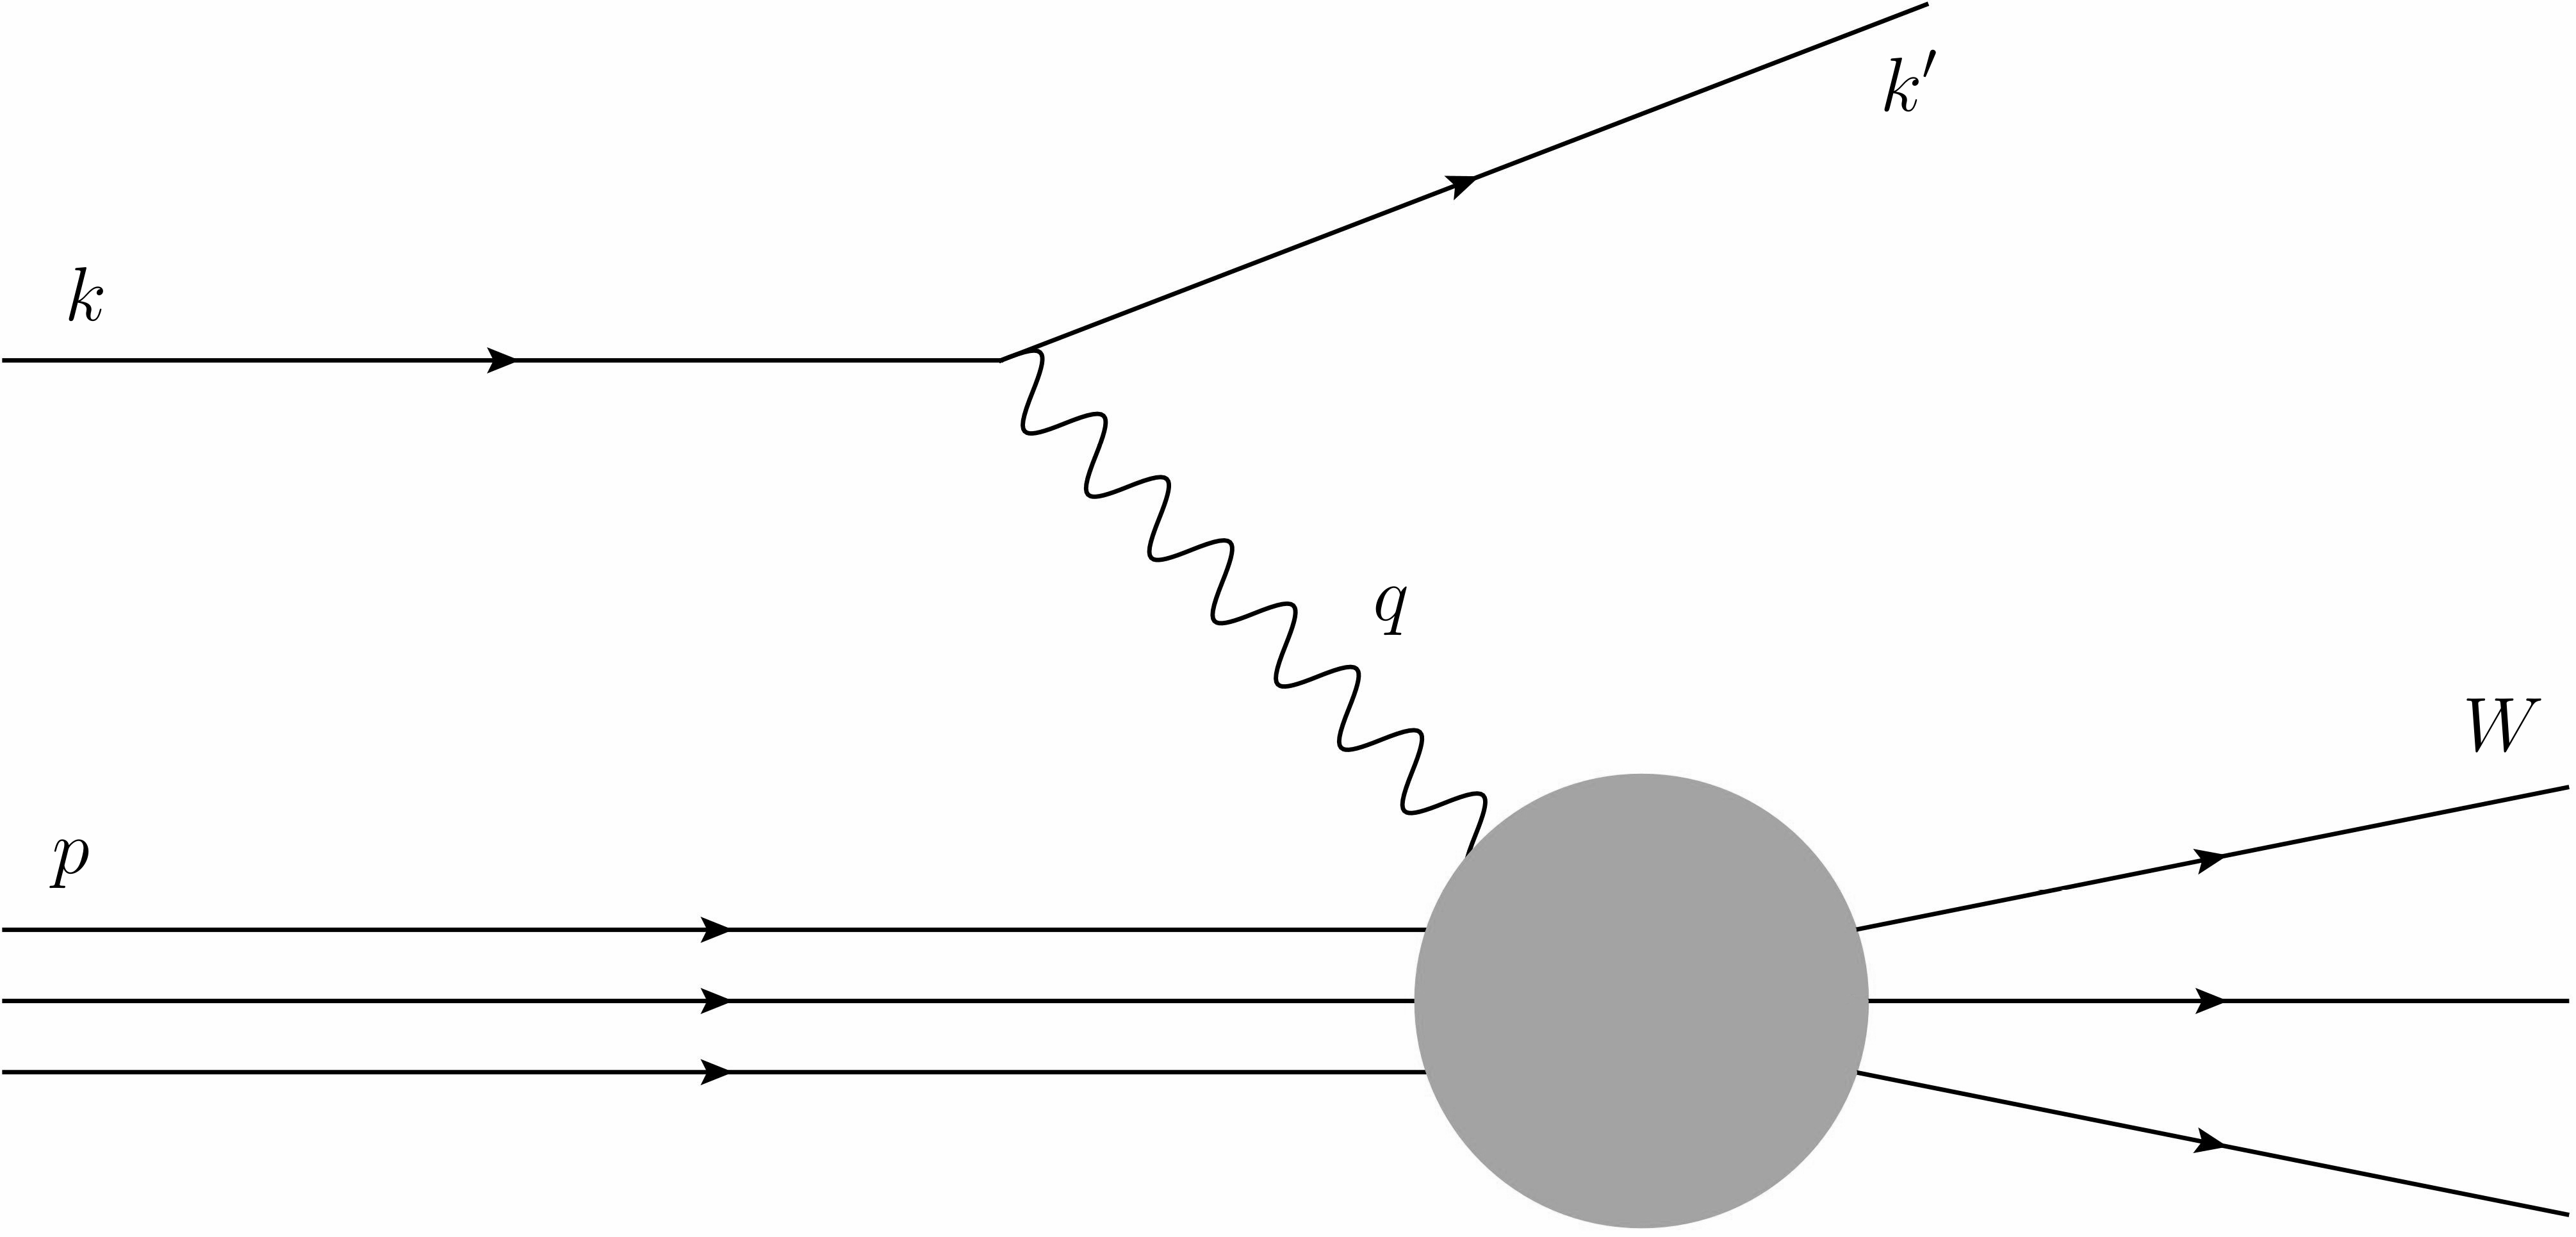
\includegraphics[width=10cm]{feyman_e_p.png}
\label{feynman}
\end{figure}
Along with $Q^2$, the variables $\nu$, W, and $x_B$  are used to narrate the evolution of the electron scattering process. $\nu$, defined as $P\cdot q/M$. Where $P$ is the 4-vector of the target proton. In the laboratory frame, $\nu$ can be described by \ref{v}. The transformation to laboratory frame allows the use of the resting nature of the target proton. Therefor $P = (Mc,\boldsymbol{0})$ and $ q = (( E-E\prime)/c,\boldsymbol{q})$. 
\begin{equation}
\label{v}
\nu = E - E^\prime{}.
\end{equation}
Simply, $\nu$ is the magnitude of energy loss by the electron during the scattering interaction. The invariant mass of the system, W,  defines the hadronic state produced by the scattering event. 
\begin{equation}
\label{W}
W^2 \equiv (q + p)^2 = M^2 + 2M\nu -Q^2.
\end{equation}
In the general case of electron scattering off of a free proton or neutron elastically, the scattered energy of the electron will be a function of the incident electron's energy and the scatted angle of the electron, shown in the following equation.
\begin{equation}
E^\prime =\frac{E}{1+\frac{E}{Mc^2}(1-cos\theta)}
\end{equation}
A scattering event with the invariant mass equal to the the mass of the nucleon, $M$, falls in the regime of elastic scattering and the final state of hadron is a recoiling proton. Increasing the $W$ above $M$ will transform the scattering interaction from an elastic scattering interaction to an inelastic scattering event due to the excited state of the scattered byproduct. 
\paragraph{} The intrinsic likelihood of an event with a certain $Q^2$, $\nu$, and $W$ is defined by the scattering cross section. An electron scattering off of a target with a charge of $Z*e$ can be described by the Rutherford cross-section. Povh et. al. details the Rutherford cross section as:
\begin{equation}
\bigg(\frac{d\sigma}{d\Omega}\bigg)_{Rutherford} = \frac{ \big(zZe^2\big)^2} {\big( 4\pi \epsilon_0\big)^2 * \big(e E_{kin}\big)^2 sin^4\big( \theta / 2 \big) }. 
\end{equation}
In the early 1920s, German physicists Stern and Gerlach performed an experiment with a beam of silver atoms. The Stern–Gerlach experiment measured the deflection of a beam of silver atoms from an inhomogeneous magnetic field\cite{strger}. The observations made by Stern and Gerlach demonstrated that particles bear an intrinsic angular momentum. In 1925, a forbidden spectral line of ionized helium raised questions of the current understanding of the quantum numbers used. This forbidden line lead to the discovery of electron spin by Uhlenbeck and Gloudsmit\cite{e_spin}. The Mott cross-section is the evolved version of the Rutherford cross-section. The Rutherford cross-section neglects the spin of an electron and the target. Evolving the Rutherford cross-section allows for the modifications needed to include the intrinsic spin of the target and electron. The Mott cross-section is described in equation \ref{Mott} \cite{HighE,PnN}.  Where $\alpha$ is the fine structure constant. This constant is related to the strength of the interaction between an electron and proton\cite{sane}.
\begin{equation}
\bigg(\frac{d\sigma}{d\Omega}\bigg)_{Mott} = \frac{4Z^2\alpha^2 \big(\hbar c \big)^2 E{^{\prime} }^2}{ |\boldsymbol{q}c|^4} cos^2 (\theta/2). \label{Mott}
\end{equation}
The inclusion of the interaction between the current of the electron and the target nucleon's magnetic moment creates the necessity to define the magnetic moment. Equation \ref{magmom} describes the magnetic moment of a charged, spin -1/2 particle. The magnetic momentum is build using M, the mass of the particle and g, a factor of 2 relating to relativistic quantum mechanics \cite{PnN}. 
\begin{equation}
\mu = g \cdot \frac{e}{2M}\cdot\frac{\hbar}{2} \label{magmom}
\end{equation}
Modifying the Mott scattering cross section equation to include a spin degree of freedom, is shown in equation \ref{spin.5}. $\tau$ is used in the cross section formalism to account for the magnetic moment of a nucleon and is defined as: $\tau = \frac{Q^2}{4M^2c^2}$ \cite{PnN}. 
\begin{equation}
\bigg(\frac{d\sigma}{d\Omega}\bigg)_{\substack{point \\ spin 1/2}} = \bigg(\frac{d\sigma}{d\Omega}\bigg)_{Mott} \cdot \big[1 + 2\tau \: \text{tan}^2\frac{\theta}{2} \big]\label{spin.5}
\end{equation}

\begin{figure}[]
	\centering
	\textbf{ }\par\medskip
	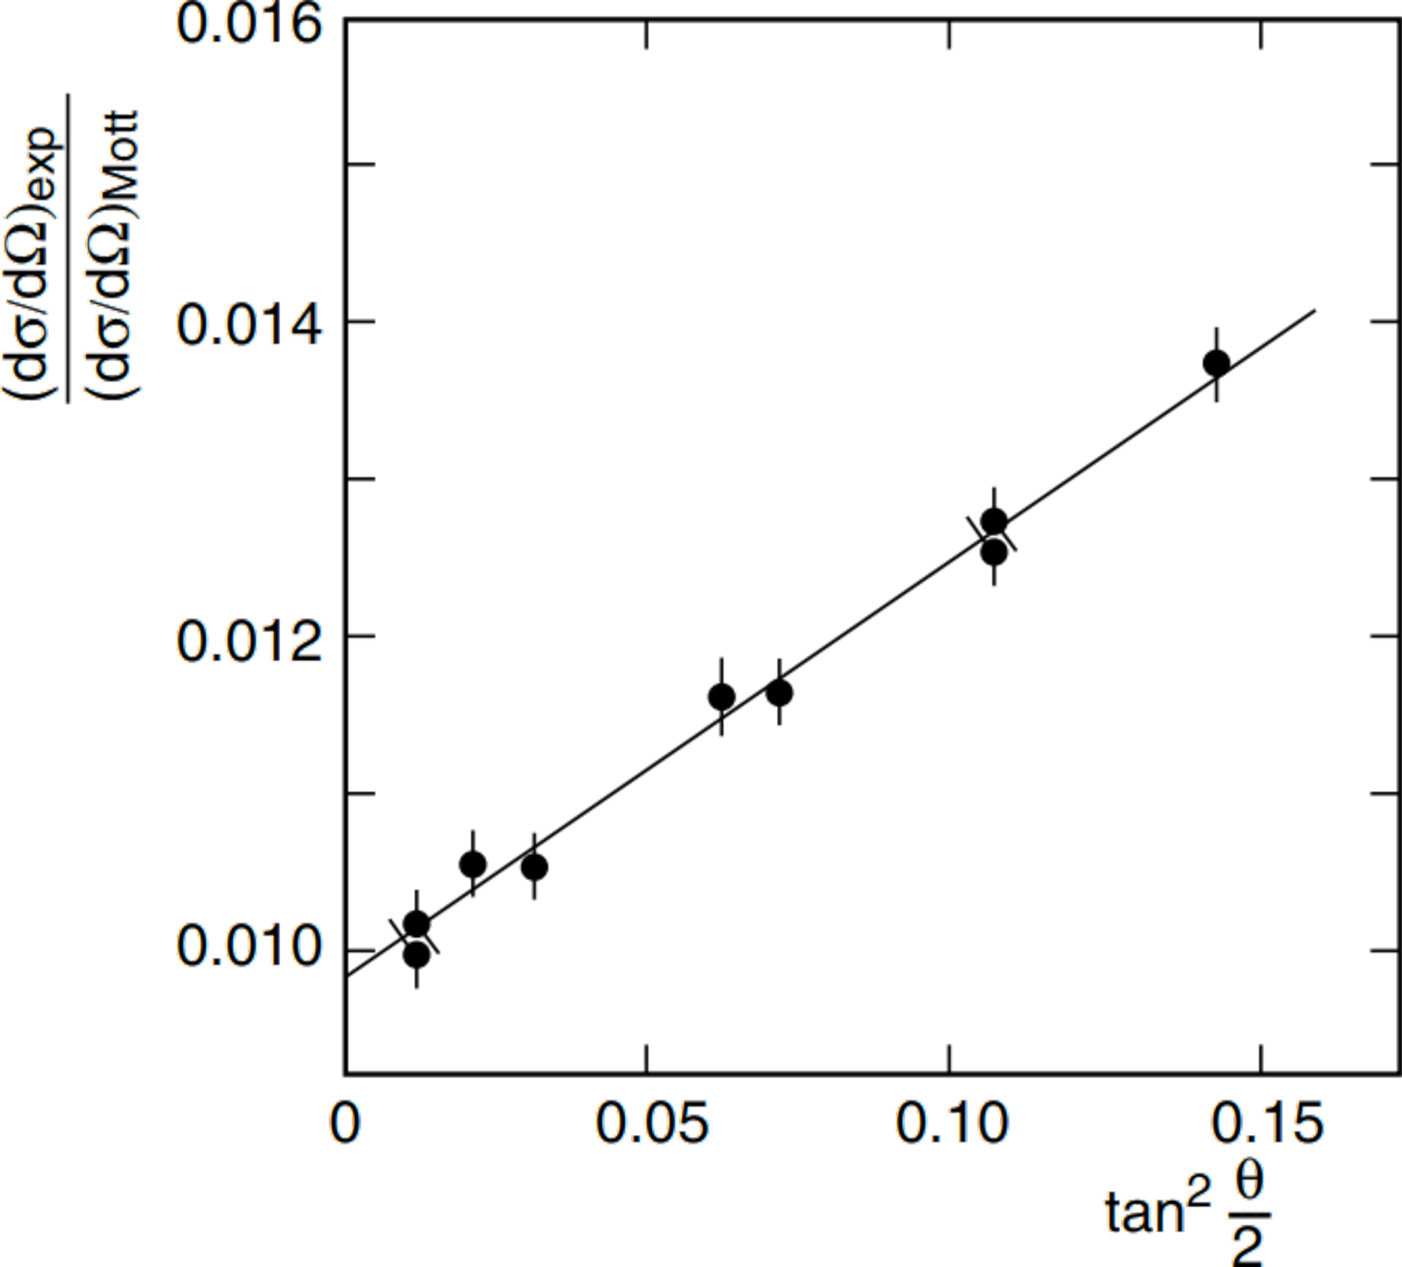
\includegraphics[width=8cm]{mott_exp.pdf}
	\caption{Ratio of experimentally measured cross section to the Mott  cross-section verses tan$^2\theta/2$ for a $Q^2$ of 2.5 GeV$^2$/c$^2$. \cite{EPinter}}
	\label{mott_exp}
\end{figure}

\paragraph{}The interaction described in the Mott cross section equation is mediated by a single photon and is electromagnetic in nature. For an electromagnetic interaction conducted at a low resolution, there is an agreement between the measured cross section and the theoretical Mott cross-section. This agreement is maximized when in the limit of $|\boldsymbol{q}| \rightarrow  0$ for scattering events of electrons off of a target nuclei. As $|\boldsymbol{q}|$ climbs furtherer from zero and the resolution of probe grows, the experimentally measured cross sections will begin to differ from the Mott cross section, systematically decreasing \cite{PnN}. The comparison of the Mott calculated cross section to experimentally measured cross section for a $Q^2$ of 2.5 GeV$^2$/c$^2$ is shown in figure \ref{mott_exp}. Increasing the $|\boldsymbol{q}|$ of an interaction reduces the size of the wavelength of the virtual photon that mediates the electromagnetic interaction between the electron and target nuclei and therefor increases the resolution of the probe. The wavelength of this virtual photon is inversely proportional to $|\boldsymbol{q}|$, and can be described by the following: $\lambda = \ \frac{\hbar}{|\boldsymbol{q}|}$ \cite{PnN}. Increasing the amount of momentum transfered in an electromagnetic reaction allows one to study deeper into the nucleus. The act of probing deeper into the nucleous or nucleon allows for the substructure of the target. 
\paragraph{} Studying the internal structure of a nucleus with the electromagnetic interaction requires increasing the momentum transfered. Pushing $|\boldsymbol{q}|$ to be comparable with the mass of a nucleon adds more complexity to the details of the scattering interaction. At the appropriate levels of $|\boldsymbol{q}|$ to study the nucleons in the nucleus, the Mott cross-section equation requires modifications to include additional factors that incorporate information about the target. The Rosenbluth formula is based on the Mott cross section and embraces target recoil, magnetic moment, and charge and current distributions. Povh writes the Rosenbluth formula as:
\begin{equation}
\label{rosen}
\bigg(\frac{d\sigma}{d\Omega}\bigg)=\bigg(\frac{d\sigma}{d\Omega}\bigg)_{Mott} *\bigg\lbrack \frac{G^2_E(Q^2) +\tau G^2_M(Q^2)}{1+\tau} + 2\tau G^2_M(Q^2)tan^2\frac{\theta}{2} \bigg\rbrack.
\end{equation}
Equation \ref{rosen} contains $G^2_E(Q^2)$ and $G^2_M(Q^2)$, the electric and magnetic form factors. These form factors depend on $Q^2$, and this measured dependence provides information on the radial charge distributions and magnetic moments of the scattering participants. For the instance of $Q^2 \rightarrow 0$, the values of  $G^2_E(0)$ and $G^2_M(0)$ are physically important.
\begin{align}
	\begin{split}
		&G^P_E(Q^2=0) = 1 \\
		&G^P_M(Q^2=0) = 2.79
	\end{split}
	\begin{split}
	    &G^n_E(Q^2=0) = 0 \\
	    &G^n_M(Q^2=0) = -1.91 \label{FFeq}
	\end{split}
\end{align}
The $G^2_E(0)$ corresponds to the electric charge of the target. $G^2_M(0)$ is simplified to the magnetic momentum normalized by the nuclear magneton. The result of $G^2_E(0)$ and $G^2_M(0)$ for the proton and neutron are shown in equation \ref{FFeq}\cite{PnN}. There were many experiments at SLAC that studied the $Q^2$ dependence of these form factors in the early seventies. The results from these form factor experiments determined that $G^p_E(Q^2) = \frac{G^P_M(Q^2)}{2.79} = \frac{G^n_M(Q^2)}{-1.91} = G^{dipole}(Q^2)$. Where $G^{dipole}(Q^2)$ is a dipole fit that describes the form factors very well\cite{PnN}.

 
\section{Deep inelastic scattering}\label{sec:DIS}
\paragraph{}The first generation of electron scattering experiments achieving a significantly large  $|\boldsymbol{q}|$ used a linear accelerator with a 25 GeV maximum beam energy, and following generations increased the total interaction energy to substantially higher thresholds. At these high incident beam energies, individual resonances cannot be separated in the invariant mass spectrum above 2.5 GeV. Observations made into this convoluted invariant mass spectrum has shown that many strongly interacting particles are produced, known as hadrons. Scattering interactions that generate these hadrons are considered to be inelastic.
\begin{figure}[]
	\centering
	\textbf{ }\par\medskip
	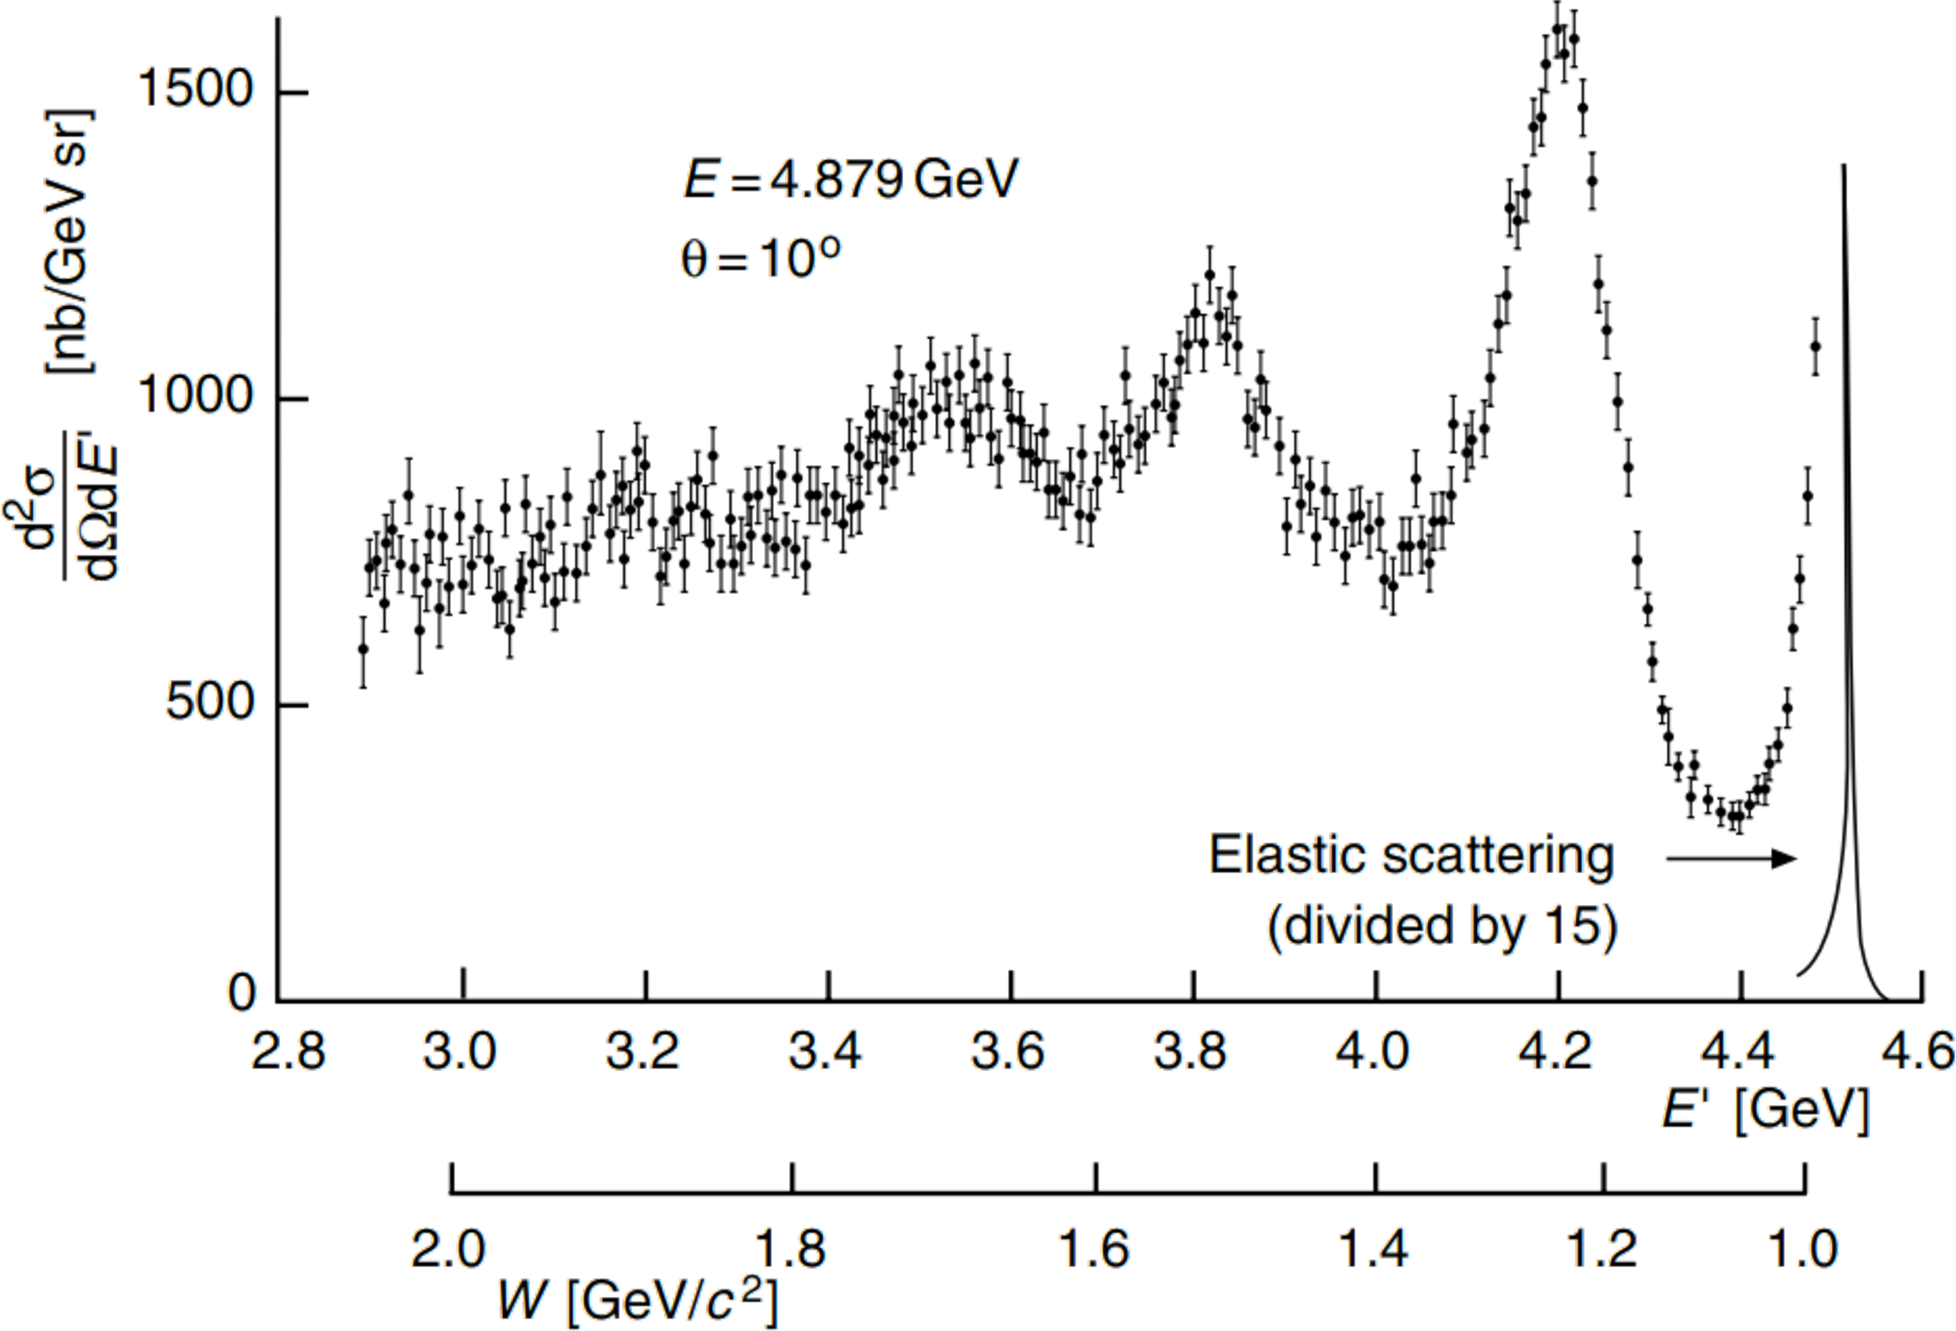
\includegraphics[width=13cm]{elasticspectrum.pdf}
	\caption{Electron-proton scattering for incident energy of 4.9 GeV and scattering angle of 10$^\circ$ \cite{deltaIsobar}.}
	\label{wspect}
\end{figure}
\paragraph{} Figure \ref{wspect} contains the invariant mass spectrum for an electron scattering from a proton target for an incident energy of 4.9 GeV  and angle of 10$^\circ$ \cite{deltaIsobar}. These results are from an experiment at Deutsches Elektronen-Synchrotron (DESY) published in 1968. The elastic scattering peak is scaled down by a factor of 15 to provide an appropriate scaling of the complete spectrum. As $\nu$ increases or the scattered electron energy decreases relative to the incident energy, the invariant mass of the scattering interaction increases. As $W$ rises, the resonance begin to convolute together. This behavior is indicative of reaching a new threshold. For scattering interactions with $W \gtrapprox 2.0 GeV/c^2$, observations are made that result in the discovery of the production of many strongly interacting particles. 
\begin{figure}[]
	%	\hspace*{-20pt}
	\centering
	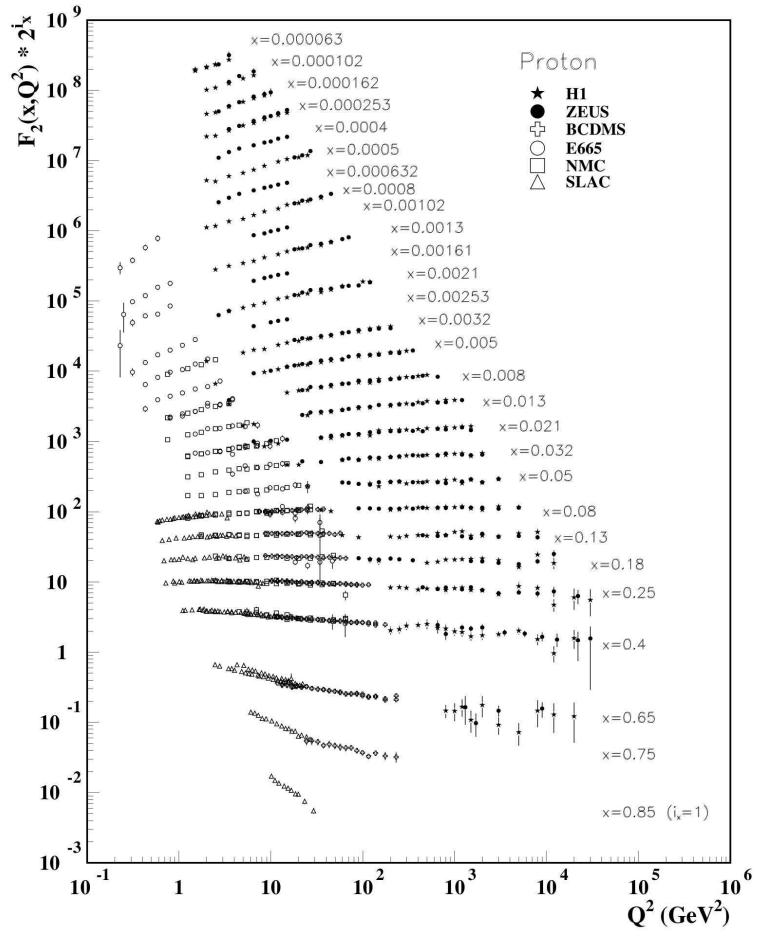
\includegraphics[width=14cm]{SLAC_F2.png} 
	\caption{ Measurements of the proton structure function $F_2(x, Q^2)$ for different $x$ settings\cite{ref:rev_pp} .}
	\label{F2_fig}
\end{figure} 
\paragraph{}Inelastic scattering events contain the possibility of conceiving additional resultants causing an increase in the complexity of a scattering interaction. In order to create an inelastic event, the wavelength of the virtual photon has to be comparable to the radius of the struck nucleon. Increasing the amount of transferred momentum so that $Q^2R^2 \gtrsim 1$, will increase the resolution of the probe to a level that allows for the interaction to be with the charge constituents within the nucleon. When the scattering event probes the fundamental elements of a nucleon, the scattering process is titled deep inelastic scattering(DIS). Due to the increase in complexity, an additional degree of freedom has to be introduced into the scattering cross section formalism. Modifying the Rosenbluth formula to include the inelastic scattering structure functions $F_1(Q^2,\nu)$ and $F_2(Q^2,\nu)$ evolves the Rosenbluth formula to contain the needed complexity of an inelastic event. These modifications are shown in equation \ref{ISCS}. The $F_1$ and $F_2$ structure functions provide the details for describing the internal composition of the nucleon \cite{PnN}. For elastic scattering events $2M\nu - Q^2 = 0$, this forces only one kinematic parameter to vary freely. However for inelastic scattering events $2M\nu - Q^2 > 0$, this creates an additional free parameter and is the reason for the  $F_1$ and $F_2$ structure functions being functions of both $Q^2$ and $\nu$.
\begin{equation}
\label{ISCS}
\frac{d^2\sigma}{d\Omega dE^\prime}=\bigg(\frac{d\sigma}{d\Omega}\bigg)_{Mott} \bigg\lbrack \frac{F_2(Q^2,\nu)}{\nu} + \frac{2F_1(Q^2,\nu)}{M}tan^2\frac{\theta}{2} \bigg \rbrack.
\end{equation}  

\subsection{Scaling}
\paragraph{}The Bjorken scaling variable, $x_B$ or $x$, is a dimensionless quantity that measures the in-elasticity of a scattering process and is defined as: $x \equiv \frac{Q^2}{2M\nu}$. Measurements from the Standford Linear Accelerator(SLAC) and others for the DIS $F_2$ structure function are displayed in figure \ref{F2_fig}. This plot displays results of $F_2$ as a function of $x$ and $Q^2$. The $x$ dependence of $F_2$ is strong and shows that $F_2$ will decrease as $x$ increases. However, at a constant value of $x$, the dependence of $Q^2$ on $F_2$ is weak for moderate values of $x$. This phenomenon of a solo dependence on $x$ was known as scaling. This scaling was observed to be present for scattering interactions with $Q^2 > 2 \: GeV^2$  and $\nu > 2.5 GeV$ \cite{Atwood}. In the Bjorken limit, v $\rightarrow \infty$ and $Q^2 \rightarrow \infty$, the deep inelastic structure functions can be described as functions of only $x$.


\subsection{Quark Parton Model}
\paragraph{}In the case of DIS off of a proton, the electron probe is used to explore the exclusive internal structure of the proton, it's constituents. In 1969, Feynman assumed the internal make up of the proton was that of point-like partons \cite{Briskin_thesis,DISproton}, the basis of the parton model. As part of this model, the impulse approximation makes an assumption that the duration of the interaction between the mediating photon and parton is relatively short, allowing for the interaction between individual partons to be neglected. Thus in a DIS interaction, the partons can be described as quasi-free, with minimal internal interactions. Under this understanding, an electron-nucleon DIS interaction would characterize the properties and motions of the partons that form the struck nucleon\cite{DISproton}.

\begin{figure}[t]
	\centering
	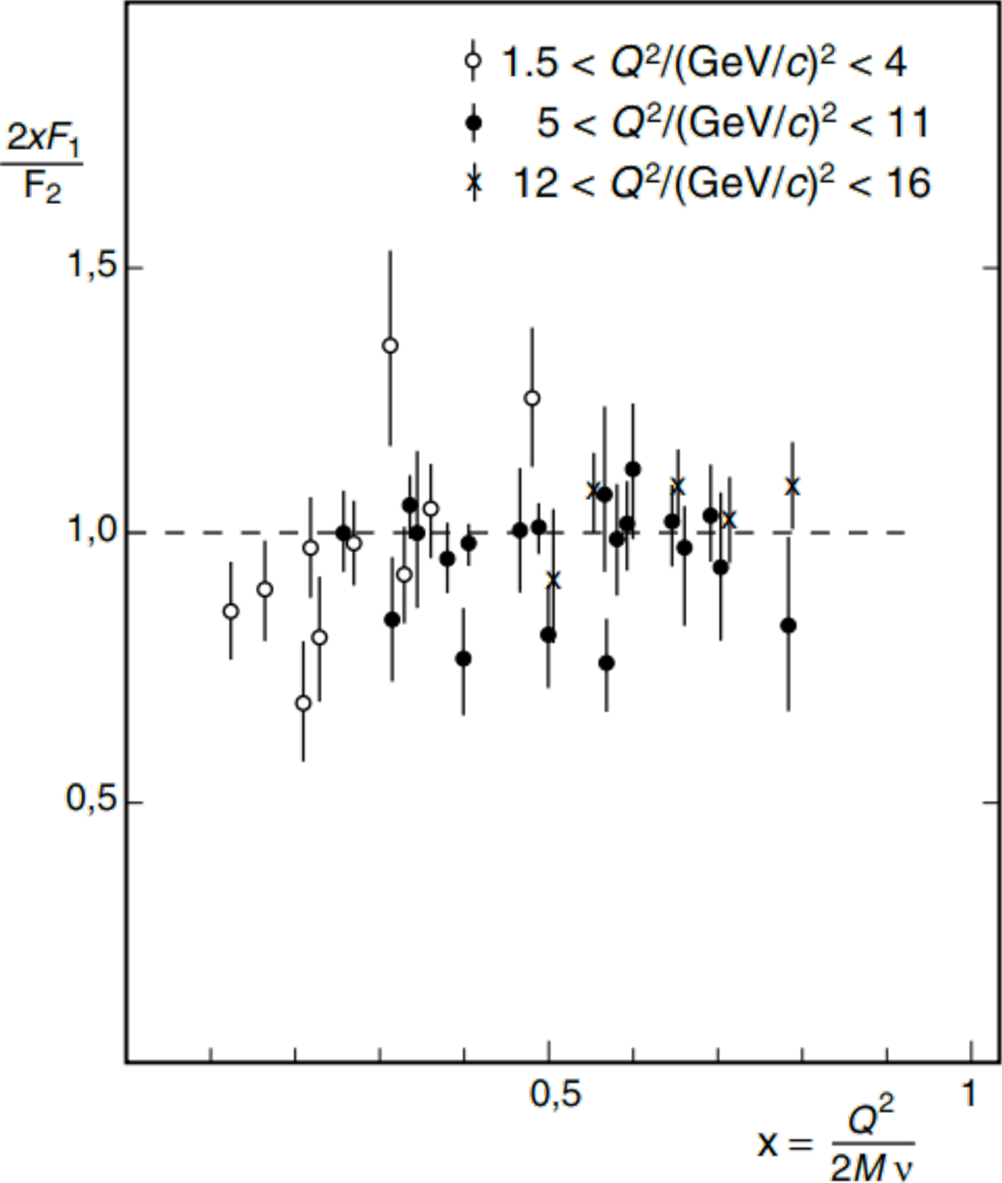
\includegraphics[width=8cm]{f1_f2_spin.pdf} 
	\caption{Data from SLAC plotting the ratio of the structure functions $2x\cdot F_1(x)$ and $F_2(x)$ vs. $x$ \cite{PnN,IntroHEP}.}
	\label{fig:spin1/2}
\end{figure} 

\paragraph{}The characteristics, (the motions and properties), of the partons are formalized into a parton distribution function $f_i(x_B)$ \cite{PnN}. The relationship for the parton distribution function with the $F_2$ structure function is shown in equation \ref{F2pd}. The $F_1$ structure function is the DIS equivalent to the magnetic form factor from equation \ref{FFeq}, and will vanish for scattering from spin zero particles \cite{PnN}. Figure \ref{fig:spin1/2} shows the linear relationship of the ratio of $\frac{2xF_1}{F_2}$ as a function of $x$. This data from SLAC helped confirmed theories from C. G. Callan Jr. and David J. Gross that the partons that are found in the nucleons of a nucleus are spin 1/2 \cite{callan,DISquark}. The relationship between $F_1$ and $F_2$ is known as the Callan-Gross relation \cite{PnN}. This relationship can be seen in equation \ref{CGr}. 


\begin{align}
		F_2(x) &= x \Sigma_i e^2_i f_i(x) \label{F2pd}\\ 
		F_1(x) &= \frac{1}{2x} F_2(x) \label{CGr} 
\end{align}
\begin{equation}
		F_2(x) = x \cdot \Sigma_f z^2_f ( q_f(x) + \bar{q}_f(x)) \label{F2quarks} 
\end{equation}
\begin{figure}[t]
	%	\hspace*{-20pt}
	\centering
	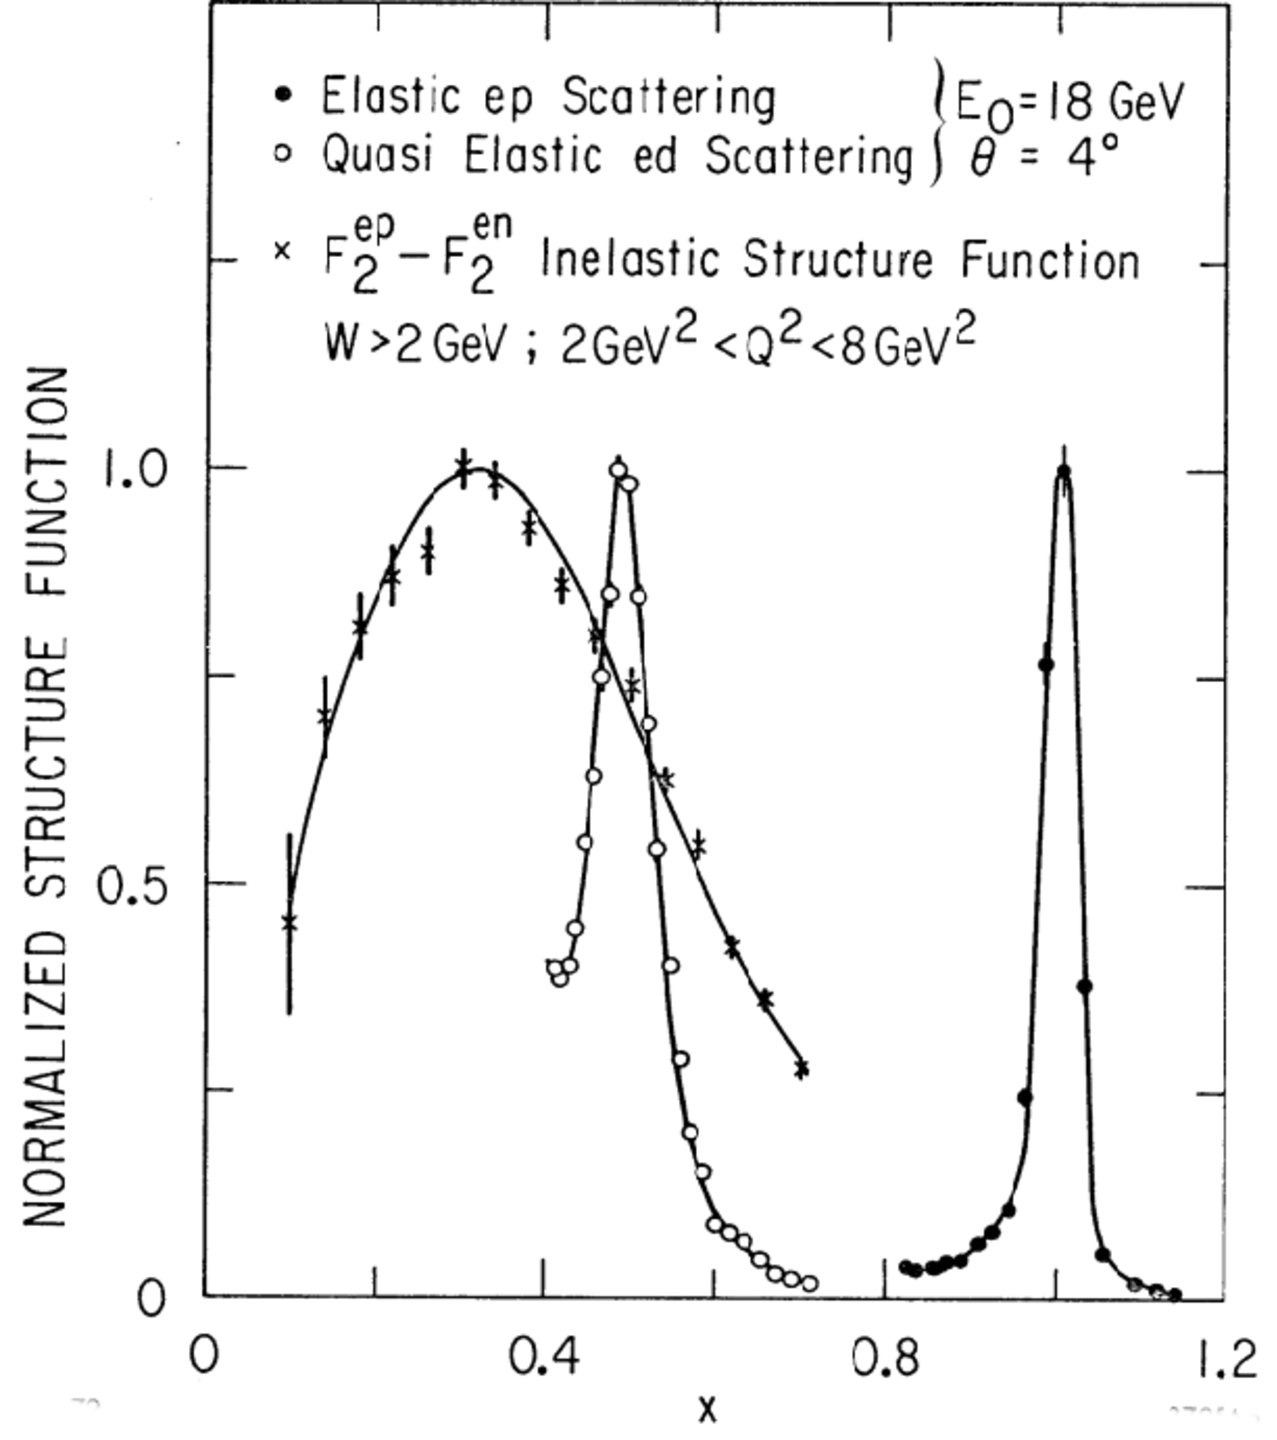
\includegraphics[width=10cm]{3slacexp.pdf} 
	\caption{ Structure function results measured from three  lepton-nucleon scattering experiments \cite{Atwood}.}
	\label{3leps}
\end{figure}
\paragraph{}The electromagnetic interaction that occurs during a scattering event happens between two charged bodies. The electron carries a charge of $- e$ and the proton carries a charge of $+e$. The partons that makeup the proton or neutron must carry a total charge equal to the charge of the proton or neutron. Using DIS scattering from electron, neutrino, and muon beams, the amount of charge carried by the partons was determined by using the equation \ref{F2quarks} \cite{PnN,DISquark,callan}. 

\paragraph{}Figure \ref{3leps} from Atwood et. al. (1982), contains data on three unique experiments plotting structure function results against $x$. Solid dots are elastic electron proton at an incident energy of 18 GeV and scattered angle of 4$^\circ$. The elastic peak at $x$ of 1 is due to the scattering event happening elastically off the entire proton. The open points are quasi-elastic scattering from deuterium. The peak is located at 0.5 in $x$ because the scattering event happens from the proton and neutron, which individually contain only half of the mass of the complete deuteron. The data represented by an 'x' displays result from an inelastic electron scattering measurement. The data plotted is the difference between two nucleon structure functions. The peak is located at one-third. The location of the peak at one-third demonstrates that the struck constituents of the nucleon have a mass approximately one-third of the nucleon and there exist three constituents inside the nucleon with equal mass\cite{Atwood,PnN}.
\begin{figure}[t]
	\centering
	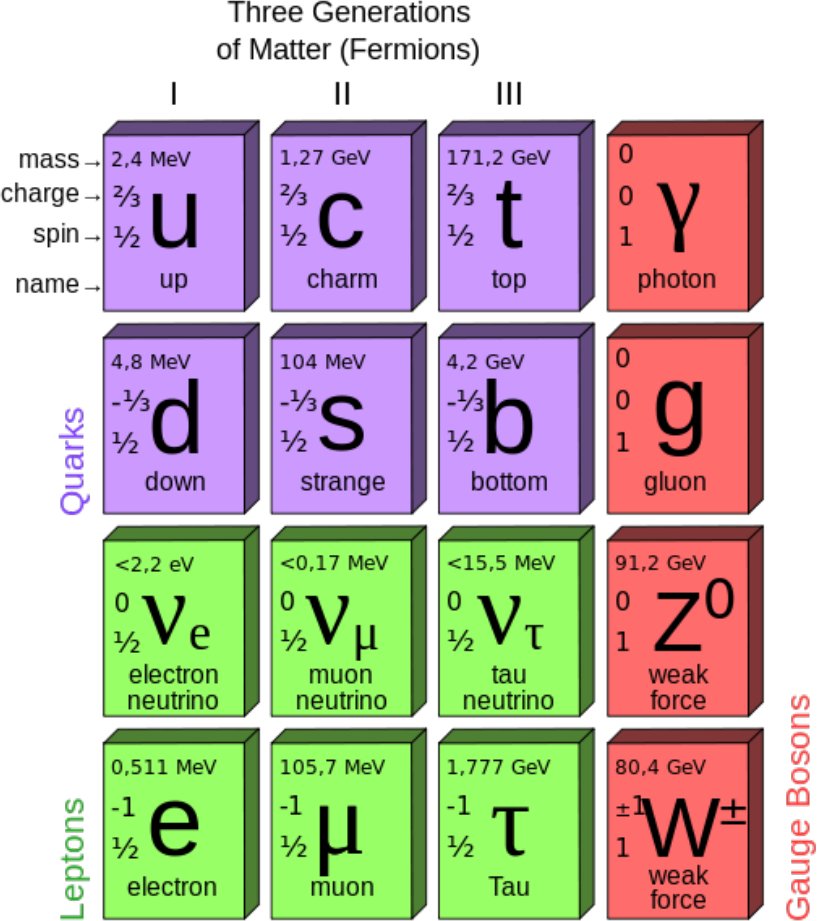
\includegraphics[width=7.5cm]{quarks.png} 
	\caption{ Elementary particles including leptons, quarks, and bosons with mass, charge, and spin \cite{sane}.}
	\label{fig:quarks}
\end{figure} 
\paragraph{}Nuclear physicist of the mid 19th century changed the understanding of the building blocks of nature by discovering fundamental constitutes of the protons and neutrons. It was unearthed that these partons have an electric charge, spin of 1/2, and some mass. Due to these partons having these properties, they can be identified as quarks from Gell-Mann's symmetry scheme, the eightfold way. This theory was based on the SU(3) mathematical symmetry \cite{strger,8fold}.
Through nuclear and high energy experiments six quarks have been discovered\cite{DISLaH}. A table of the elementary particles is shown in figure \ref{fig:quarks}.
%\paragraph{}The quarks that make up the nucleons, two up quarks and one down quark for the proton or two down and one up for the neutron, only contains half of the total momentum of the nucleon. Part of the remaining momentum is carried by particles identified as gluons which do not interact electromagnetically or weakly\cite{PnN}. The internal structure of a proton is not only made up of the up and down quarks (the valance quarks) and gluons. There are also quark-antiquark pairs that carry a small fraction of the momentum. These quark-antiquark pairs are known as the sea quarks.
\paragraph{}A scattering interaction between a lepton probe and a target nucleus probes the structure of the target. A DIS interaction delves inside the nucleus to observed the nucleons and their quarks and gluons. The European Muon Collaboration (EMC) used DIS experiment to study the internal structure of a few targets. Their use of DIS in 1983 discovered a new phenomenon defined as the EMC effect \cite{PnN,CC}.
